\section{Viscous: Protocol Descriptions}
To overcome the limitations of existing transport layer protocols as discussed in the previous section, we propose a new transport protocol called Viscous. It is a connection oriented multipath multi-flow transport protocol which is not coupled with the network stack, and work as a wrapper or a middleware between the users' application and the transport layer of the network protocol stack. The basic design philosophies for Viscous are as follows. 
\begin{enumerate}
	\item To mitigate the signaling overhead associated with connection establishment, Viscous multiplexes multiple flows over a single Viscous connection. This reduces the connection setup time for short-lived flows. 
	\item Viscous does not maintain a separate and independent congestion control for every application flows. Rather, it maintain a single congestion control mechanism for a Viscous connection which is a multiplex of multiple flows. Further, the congestion control is path specific, that is, congestion is monitored at every path from a source to a destination, where a Viscous sub-flow is initiated.  
	\item Viscous follows a modular architecture for ease development of applications. Any Viscous module can be tuned independently to make it suitable for a specific performance bound. This way, application layer quality of service (QoS) can be provided with the help of Viscous. 
	\item Viscous works on top of UDP, similar to Goggle's QUIC; therefore it mitigates the transport layer protocol overhead which is associated with TCP. 
	\item Viscous supports different types of mobility without breaking an existing connection. With the help of a unique client and server specific identifier which is shared during the initial connection establishment, Viscous can continue with the existing connection, even if the server or the client changes its IP address.   
	\item Viscous follows a layered architecture with two different layers, as shown in Fig.~\ref{fig:sys-io}. The top layer consists of multiple flows from various applications, and the bottom layer consists of multiple channels, corresponding to each path between a server and a client. To avoid the signaling overhead from the connection establishment and the slow-start phase, congestion control and reliability are associated with the bottom layer which consists the channels. On the other hand, flow-control and data transmission are designed as a part of the upper layer, which is associated with the flows.
	\item Consequently, Viscous decouples the congestion control from the flow control. This helps in avoiding slow start for all the flows between a source and a destination, those share common paths end-to-end. The flow control is kept flow specific, whereas the congestion control is kept channel or path specific. 
\end{enumerate}



\begin{figure}[!ht]
	\centering
	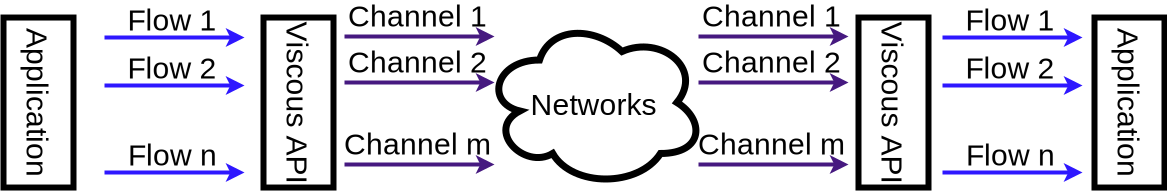
\includegraphics[width=\linewidth]{img/sys-io}
	\caption{Flow-Channel architecture in the Viscous protocol. Application sends and receives data through the flows. Internally, Viscous sends and receives data using multiple channels over multiple paths.}
	\label{fig:sys-io}
\end{figure}



%\acrshort{tcp} suffers for short-lived flow because of slow-start and connection establishment time. To mitigate this problem, we multiplexed multiple flows over a single viscous connection similar to \acrshort{quic}. 

%
We develop Viscous as a software library for Unix type systems. We implemented the entire protocol in the user space, and therefore we do not require any change in the existing Kernel or the TCP/IP protocol stack. In this section, we first discuss the fundamental concepts behind the development of Viscous and then talk about various internal protocol details for Viscous implementation.
%
\subsection{Key Concepts Behind the Design of Viscous}
There are two key concepts behind the design, development, and implementation of Viscous to support ubiquitous transport of data over any Internet devices -- \textit{flow} and \textit{channel}. These two concepts are the input and the output of the Viscous module, as depicted in Fig.~\ref{fig:sys-io}.

\subsubsection{Channel}
Channels are individual connections between two devices over multiple paths. There is one single channel for each path. To avoid connection time path imbalance like MPTCP, as we observe in Fig.~\ref{fig:timeSentOverPath}, we initiate all the channels simultaneously after connection establishment and before any flows can start. Connections are established specific to a destination host whenever an application from a source host requests for a connection. This connection is shared with other applications which intend to send data to the same destination host. This way, flows are multiplexed specific to a destination host. A common example for such scenario is the IoT gateway applications, where multiple sensor nodes transfer data to a destination gateway via a common source gateway. In Viscous, flows do not require connection establishment as the connection has already been established between the source and the destination. Viscous handles congestion control for every individual paths between a source and a destination. Therefore, flow specific congestion control is not required for Viscous, and Viscous maintains path specific congestion control. This way Viscous avoids slow start for every individual flows that share the complete path from the source to the destination. Consequently, channels are persistent in Viscous, and they do not die out after the completion of a flow. As mentioned, a channel can carries data from multiple flows simultaneously by multiplexing them. If one or both the devices are multi-homed, multiple channels can be established that share the traffic load and therefore, achieve better performance.

\subsubsection{Flow} 
Flows in Viscous are responsible for data communication while maintaining the flow-control between a source and a destination. An application can transmit data over multiple flows simultaneously. The user application sends data as byte-streams to the flow, and it also receives data in the form of byte-streams from a flow. Flow is responsible for packetizing the byte-stream and sending the packets to the lower layer of Viscous. We do not put congestion control inside a flow because it is not persistent and we do not want to go through the same slow-start phase again for multiple flows between a source and a destination. So, Viscous puts packets from flows to channels, and the channels take care of the congestion control. This way, we decouple congestion control from flow control in Viscous design. 

This channel-flow decoupled architecture gives Viscous the power of utilizing multiple paths even for short-lived flows. Flows do not have to suffer from slow-start or connection establishment overhead. The connection establishment is a separate event from channel management, and all the channels between a source and a destination start simultaneously. This removes the problem of path selection as we observe in MPTCP.  Further, channel gives an option to support mobility. If one or both the devices change its network address, the associated channel cannot communicate anymore. Viscous can discard the affected channels and initiate new channels using the new network address without any interruption in Viscous connection (application flows). 


\subsubsection{Channel Scheduler}
Viscous channel scheduler schedules packets from application flows to one of the channels. A straightforward way  to schedule the packets is to allocate channels to the packets in a round robin way. However, round robin channel scheduling is not optimal because different channels can have different network characteristics in terms of bandwidth, delay or packet loss; as they are associated with different end-to-end paths in the network. Therefore we use an acknowledgement (ACK) driven scheduling for Viscous, that works as the base scheduler. Here the scheduler schedules a packet to a channel when it receives the ACKs corresponding to the already transmitted packets in the channel. Whenever the scheduler receives an ACK over a channel, it schedules the next packet to that channel. This provides a self-clocking behavior to the channel scheduler. This way, Viscous resolves the issue of balancing packets among various channels.

It can be noted that this is the base scheduler that we have designed for Viscous. The scheduler can be extended to support application QoS, where different flow may require different bandwidth. This provides design flexibility to Viscous, where an application programmer can control Viscous modules for applications' need.  

%The real power of Viscous lies in $flows$. An application will communicate with remote applicate using a flow only. The application can run multiple flows simultaneously without blocking other flows. Flow can start to send data without spending any time in connection establishment and may not have to go through the slow-start phase. Flows allow an application to transmit byte-stream from one application to remote application. Flows are responsible for packetizing byte-stream and send the packet to lower layer. It is also responsible for reordering unordered packets received from the lower layer and send byte-stream to the application. Flows are not liable for reliable transmission or congestion control as \textit{channel} handles these things. However, it should provide flow control mechanism.

%\subsubsection{Interface Id} Viscous mark every network interface available in a device by a 4-bit nonzero positive integer. For now, we only support maximum 15 interfaces (although never tested with 15 interfaces).

%\begin{figure}[!h]
%    \centering
%    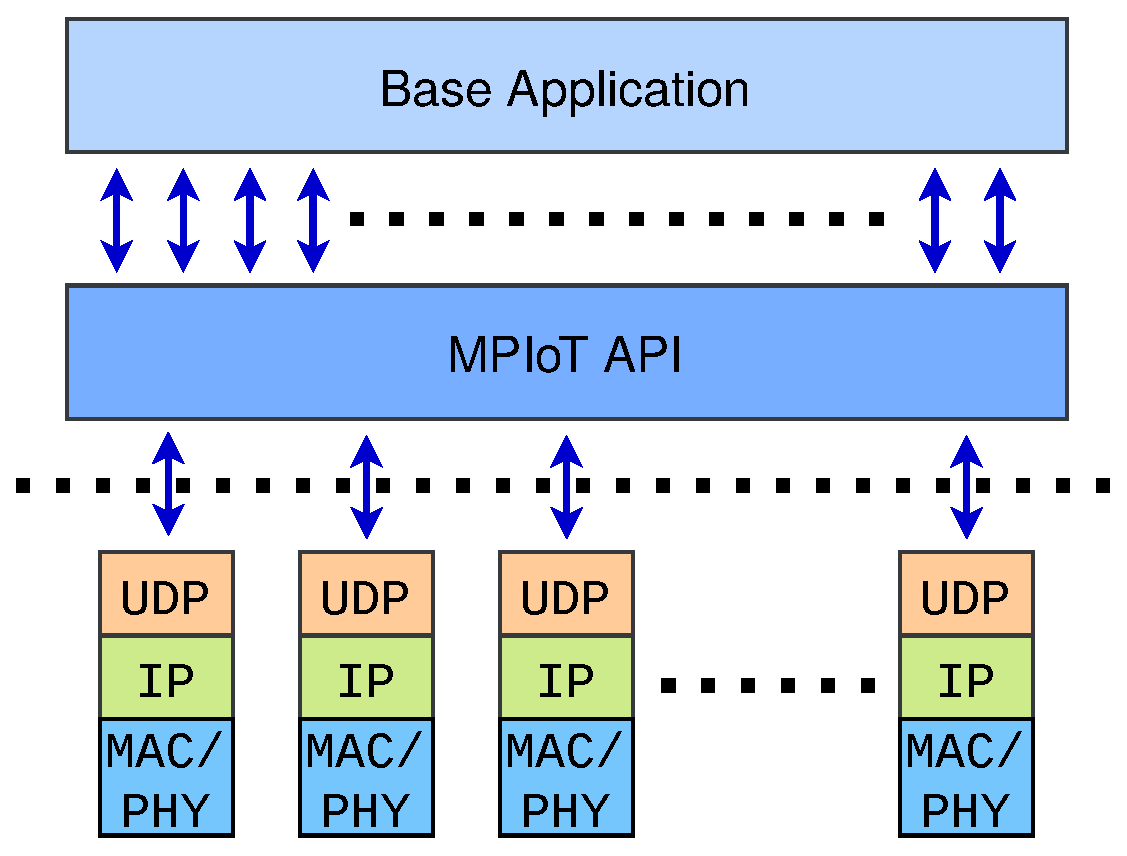
\includegraphics[width=.65\linewidth]{img/sysArch}
%    \caption{}
%    \label{fig:sysArch}
%\end{figure}


%\subsubsection{Channel} 
%Channel is an internal method Viscous uses to communicate to a remote Viscous enabled application. Flows are internally multiplexed and send through one or more channel. Each distinct source-interface and destination interface pair can one channel. Channels are expected to provide reliable transmission between two application. It is also responsible for handle congestion in the pipe. An application can not use channels directly to transmit data. Creation of channel is implementation dependent. There is no requirement of any handshaking during the channel creation. However, it is needed to check if a channel can be established or not. It may happen that, there is no path between one interface-pair.


Viscous is a connection oriented protocol. So it uses the client-server architecture for creating and maintaining the connections. A Viscous server waits for a new connection from a Viscous client. One Viscous server can stay and manage connections with multiple clients. For each client connection, the server maintains separate sets of channels and other associated modules. This separation of channels is required as the different clients may follow different paths from the server. 

%
%\subsubsection{Viscous Server}
%Similar to \acrshort{tcp} server, a viscous server waits for clients to connect to it. The client connects using three-way handshaking method similar to \acrshort{tcp}. 
%%
%\subsubsection{Viscous Client}





\subsection{Protocol Description}
Like every connection-oriented protocol, the life-cycle of Viscous also starts with the connection establishment state.
Other states of this protocol are -- ready to create flow,  ready to close, and  connection closure.
%Figure \ref{fig:ProtocolLifeTime} depict life cycle of viscous.
In Viscous, communication is possible only after association of the flows to the connections. Accordingly Viscous maintains the above four states as discussed next. Fig.~\ref{fig:ProtocolDiagram} shows the protocol diagram for Viscous. 

\begin{figure}[!ht]
	\centering
	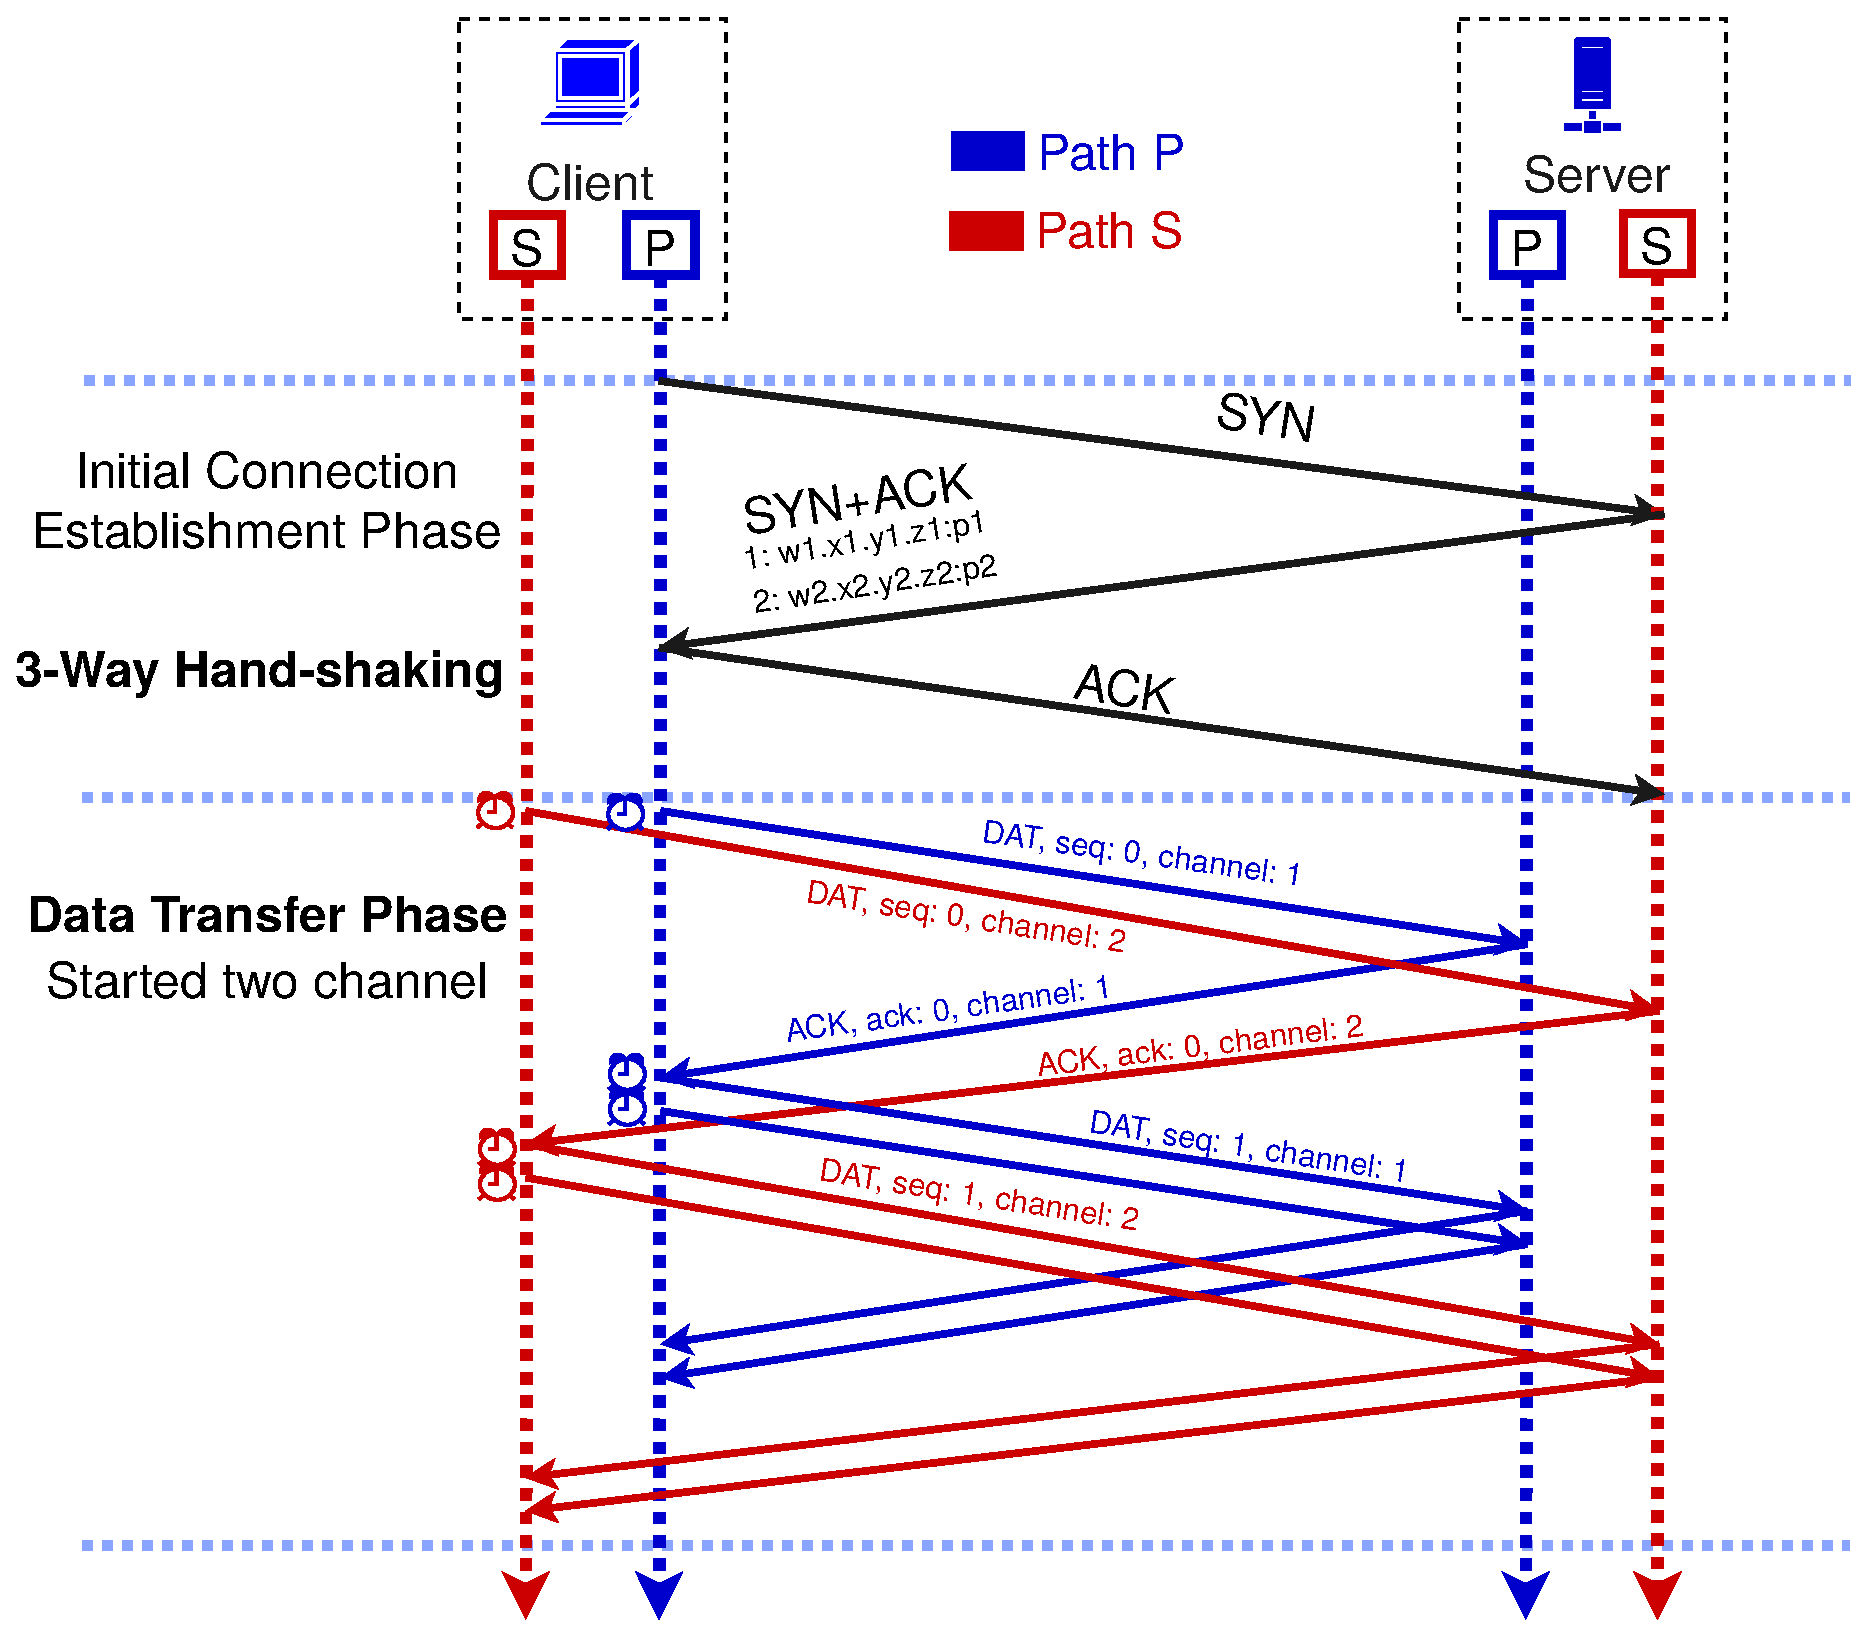
\includegraphics[width=1\linewidth]{img/ProtocolDiagram}
	\caption{Three way handshaking between client and server and data transfer between them. Handshaking can go between any two pairs of interfaces.}
	\label{fig:ProtocolDiagram}
\end{figure}

%\begin{figure}[!h]
%    \centering
%    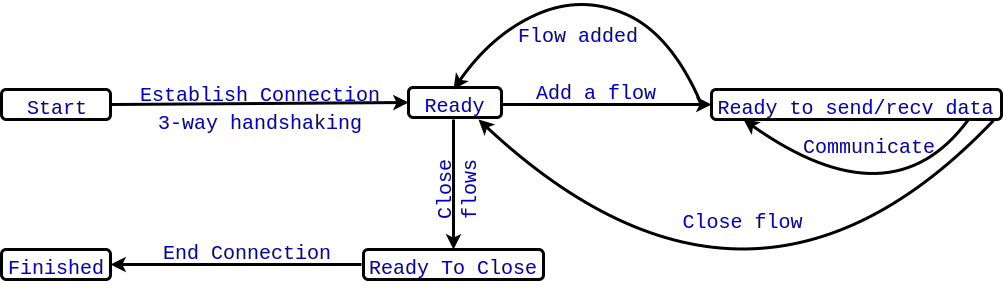
\includegraphics[width=1\linewidth]{img/ProtocolLifeTime}
%    \caption{}
%    \label{fig:ProtocolLifeTime}
%\end{figure}

\subsubsection{Connection Establishment}
We keep this procedure similar to the TCP connection establishment procedure that follows a three-way handshaking mechanism. However, as mentioned earlier, connection establishment in Viscous is in between a Viscous server and a Viscous client which is one time and does not depend on the number of flows between the same server-client pair. To establish a connection, the Viscous client sends a synchronization (\texttt{SYN}) packet with a temporary unique identifier. We can use the MAC address or the IP address of the client as this identifier. On receiving the \texttt{SYN} packet, the Viscous server generates a fingerprint for the client and sends a \texttt{SYN+ACK} packet containing the generated fingerprint. This fingerprint is used as the connection identifier for the server-client pair , and every packet between the server and the client includes this fingerprint. In our implementation, we use a SHA256 has function to generate the fingerprint from the client MAC, server MAC and the current time-stamp used as a unique nonce. It can be noted that different fingerprint is used for different connections, and therefore a fingerprint can uniquely identify a path between a server-client pair.  The connection establishment procedure ends with the Viscous client sending an \texttt{ACK} packet.
%\begin{itemize}
%    \item \textbf{SYN}: Synchronisation flag similar to \acrshort{tcp}. Indicate receiver that connection is being synchronized.
%    \item \textbf{ACK}: Acknowledgement flag. Indicator to the receiver that packet acknowledges previously received data or other packets.
%\end{itemize}

%The fingerprint is a unique identifier for a client generated by the server. 
%It is required in this protocol as this protocol can not use IP-Port tuple as client identification. 
%Viscous is a multipath protocol; each interface will have different IP-Port tuple.
%A fingerprint is the better way to identify connection when packets are going through various path/interface.
%
%Temporary unique identification is client's identification before it received any fingerprint. 
%It is required to identify a client in case of $SYN+ACK$ packet got lost, and client needs to resend the $SYN$ packet.
%We do not want to rely on this identifier for further communication because the client generates it, and any other clients may generate the same identifier by mistake or intention.

A packet loss during the connection establishment is detected using timeout. If ACK is not received within the predefined period after sending a \texttt{SYN} packet, the sender (client or server) retransmits the packet again. In our implementation, we use a timeout value of $1$ second for retransmitting a \texttt{SYN} packet, and a device can retry up to three times. During the connection establishment, the Viscous server informs all its network addresses to the Viscous client, if the server has multiple interfaces. So, immediately after the connection establishment at one channel, the Viscous client initiates all possible channels to the Viscous server. There is no requirement to send an extra control packet to complete the channel establishment. 
%Channel establishment will automatically complete when server side receives first packets of a channel from a client.
After connection establishment, Viscous clients become ready to add flows to the channels, and initiates the data transmission as the applications send data over the flows.

\subsubsection{Ready State}
Once connection got established, bothe the Viscous client and the Viscous server become ready to transmit or receive data by creating flows from the applications. We say that the Viscous protocol is under \textit{Ready} state at this phase. In this state, the Viscous channel scheduler schedules flows to the channels based on data generation from the application. 

\subsubsection{Connection Closure}
When an application has finished all the transmissions with the remote application, the application can close the Viscous connection. Connection closure in Viscous is implementation dependent, and we use TCP type connection closure at every channel that was established between the server and the client. 

\begin{comment}
\subsection{Layers in Viscous}
The Viscous protocol has multiple layers. Each layer is responsible for a different task. We are going to discuss each layer now in a top-down approach.
\subsubsection{Top layer or \acrshort{api} layer}
Top layer or \acrfull{api} layer is the layer when application directly interacts with Viscous protocol library. This layer defines how an application will interact with the protocol \acrshort{api}. It can be defined as application layer also.
\subsubsection{Flow layer}
Flows are defined in this layer. After connection establishment, an application will create one or more flows to transmit data. Data transmission between applications through flows is handled. This layer is responsible for flow control and packet reordering. There will be a multiplexer-demultiplexer at the bottom of this layer. This multiplexer-demultiplexer is liable multiplex packet arrived from different flows and sent to the lower layer and vice-versa.

\subsubsection{Channel scheduling layer}
When Viscous have multiple channels, it is needed to schedule packets to one of the multiple available channels. Channel scheduling layer responsible for this task. It is one of the important layers. Scheduling job is critical. An optimized schedulers can increase performance by reducing out-ordered packet, jitter, and delay. 

\subsubsection{Channel layer}
Channel layer is the most important layer in Viscous. This layer is responsible for taking a packet to remote device/application reliably, efficiently and equitably with other traffic in the network. This layer needs to handle congestion in a network. We do not suggest any new congestion control mechanism. \acrshort{tcp} provides multiple congestion control algorithm. Implementation can borrow any congestion control algorithm from \acrshort{tcp} and implement here. One of the important tasks of the channel layer is sent a packet through proper interface. How does an implementation can send a packet through an interface is implementation dependent. The only requirement here is, a channel should be able to forward packet to predecided particular interface and packet should reach a pre-decided specific interface at the remote device. To do this implementation may add one more layer to handle interface.

Novelty in our protocol approach is that it does not suffer from head-of-the-line blocking problem. We achieved it by separating packet reordering, flow control and congestion control in two layers. Channel layer only takes care of the congestion control. It does not store any packet it receives. Instead, it just forwards them to flow layer. Channel only keep track of the received packet in the form of a bitmap to provide reliable data transmission.

The flow layer is responsible for packet reordering and flow control. The flow layer does it individually for each flow. So, if a packet loss for one flow, it does not affect other running flows.

%\begin{figure}[!h]
%\centering
%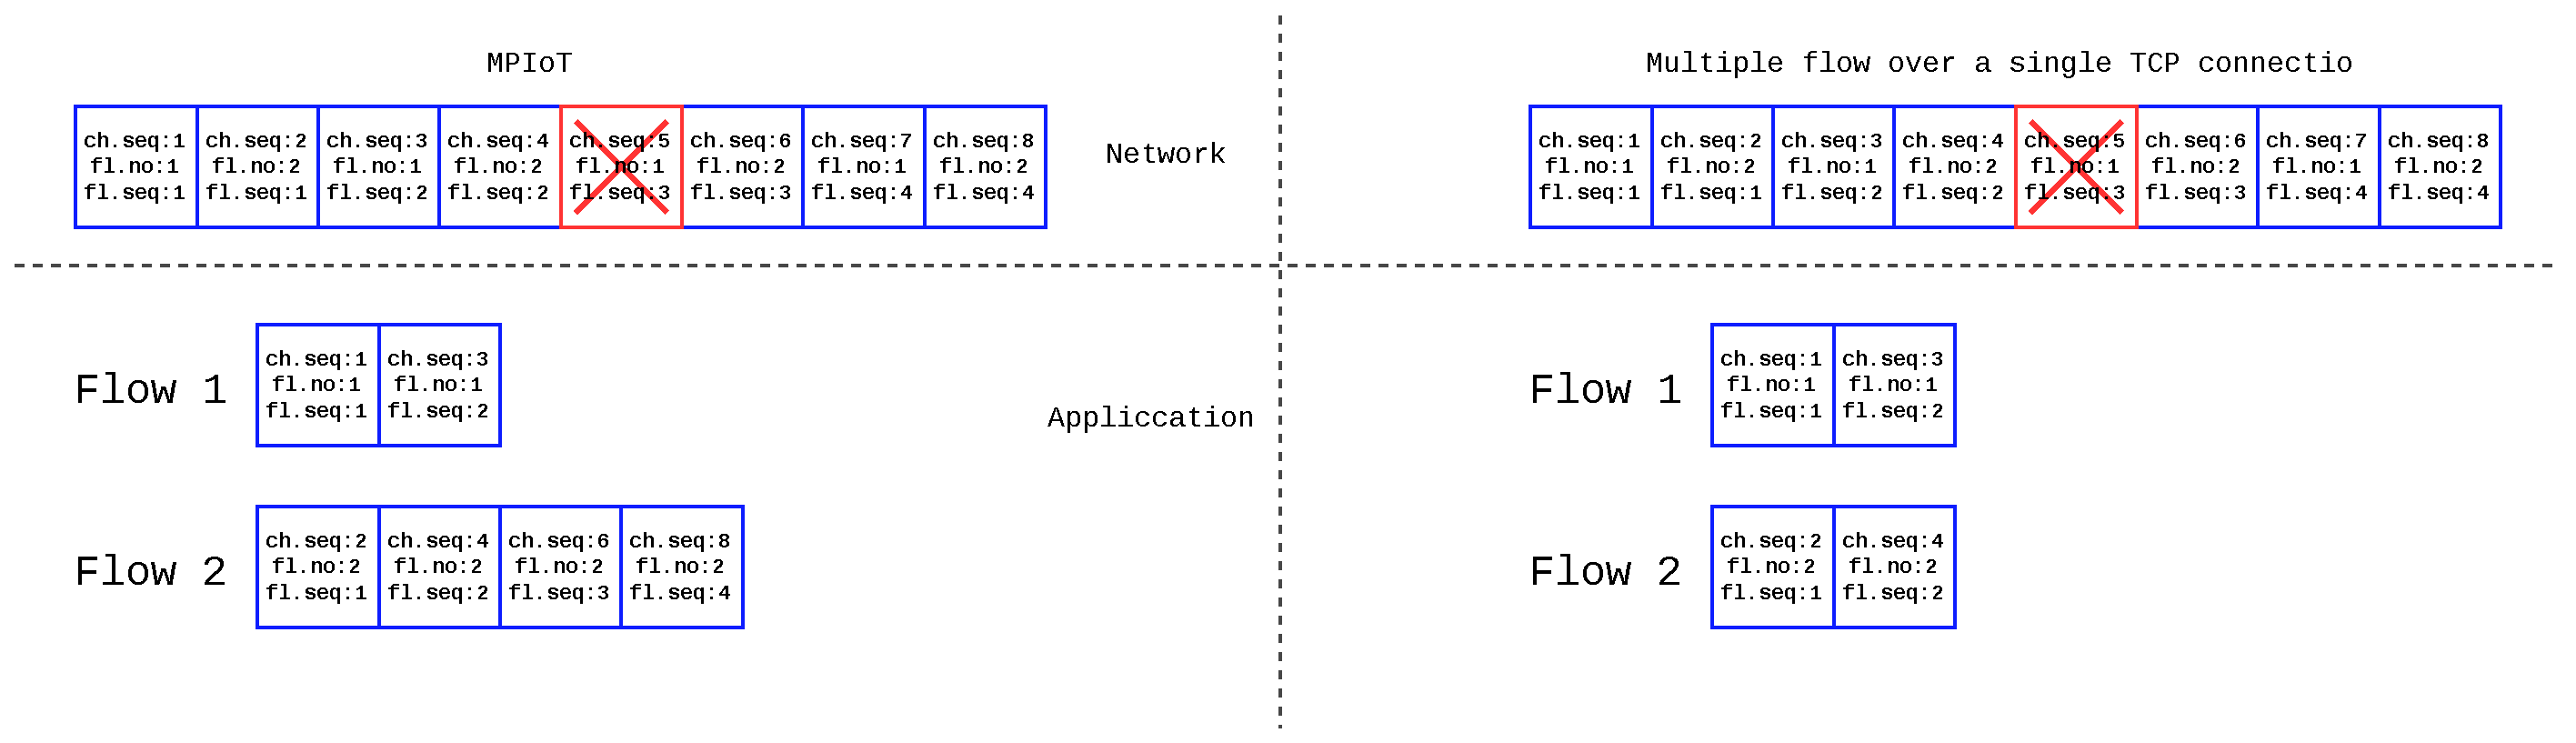
\includegraphics[width=\linewidth]{img/HOL-unblocked}
%\caption{}
%\label{fig:HOL-unblocked}
%\end{figure}


%In figure \ref{fig:HOL-unblocked}, we described how HoL blocking works for \acrshort{tcp}.
\end{comment}

\subsection{Mobility Support in Viscous}
Viscous can support different types of mobility events, as follows. 

\subsubsection{Connect-time Mobility}
A connection can fail whenever the server or the client changes its address in between the connection establishment time. With the help of a global name server, this type of mobility can be supported in Viscous. A name server is required to get the new address of the server, when the server changes its IP address. There are two cases that needs to be handled. 
\begin{enumerate}
    \item \textit{Client changes its address just after sending a \texttt{SYN} packet, Server changes its address just after receiving a \texttt{SYN} packet}: This type of failure is automatically recovered by subsequent retries from the client. During the retry, the Viscous client is identified via temporary unique identifier which is used to generate the fingerprint.
    \item \textit{Client or server changes its IP address after receiving the \texttt{SYN+ACK} packet from the server}: As \texttt{SYN+ACK} packet contains the fingerprint, the client can send the \texttt{ACK} packet to complete the three-way handshake by sending the \texttt{ACK} packet to the new server address. The new server address is received with the help from the global name server. However, the success depends on how fast the global name server can update the server IP address against its domain name. If this process fails after three retries, the client re-initiates the connection. 
\end{enumerate}

\subsubsection{Individual Mobility}
Individual mobility event occurs when one of the interfaces from both the devices change its network address. This type of mobility can affect a Viscous connection, only if the affected channel already has some packets under transmission. The subsequent packets will carry the new address to the remote device. This does not create a problem, because the connection is identified by the unique fingerprint between the server and the client. 

Further, the new IP address can be forwarded via other unaffected channels. If all the channel fails, the the affected application can take help from the name-server to find out the new address, and the new channels are creates based on that.

\subsubsection{Simultaneous Mobility}
Simultaneous mobility is rather complex, which occurs when all the interfaces of the server or the client change their network addresses simultaneously. In this scenario, the remote application is not reachable at all. In this event, all existing channels are affected. Therefore, the application needs to get the remote addresses from the name server. Once it get the new addresses, Viscous can continue with the existing connections as the fingerprint remains unchanged.
